When describing rotating particles it is common to use the so-called Euler angles $\mathbf{E} = (\phi, \theta, \psi)$. A formal definition is given by Diebel \cite{Euler} but for the purposes of this thesis we will describe them as a transformation from our stationary coordinate system $\{x,y,z\}$ to the coordinate system attached to our particle $\{x',y',z'\}$. This transformation is performed in three steps by using the intermediate axis T.

\begin{itemize}
\item Rotate the $x$-$y$ plane $\phi$ radians about the $z$-axis.
\item Denote the shifted $x$-axis $T$ and rotate the $z$-$y'$ plane $\theta$ radians around the $T$-axis
\item Rotate the $x'$-$y'$ plane $\psi$ radians around the $z$' axis.
\end{itemize}

This is illustrated in figure \ref{fig:eulerangles} where each prime marks one additional step of rotation to the coordinate system. Figure \ref{fig:eulerparticle} shows the Euler angles for a triaxial particle from a point of view similar to that of the experiment where the $x$-$z$ plane is the field of view. Note that although $\psi$ has an impact on the particle dynamics, we cannot observe it in our experiment as the particles are too symmetric around that axis, as is shown in section \ref{sec:particle_improves}


\begin{figure}[H]
\centering
\begin{subfigure}[b]{0.45\textwidth}
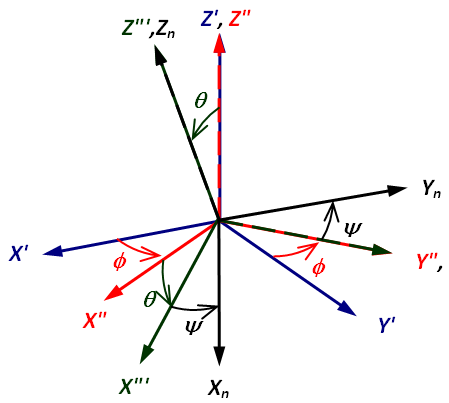
\includegraphics[width=0.9\textwidth]{figures/theory/eulerangles.png}
\caption{A general illustration of the Euler angles}
\label{fig:eulerangles}
\end{subfigure}
\begin{subfigure}[b]{0.45\textwidth}
\includegraphics[width=0.9\textwidth]{figures/theory/EulerAngles.pdf}
\caption{The Euler angles as used in our experiment}
\label{fig:eulerparticle}
\end{subfigure}
\caption{Figure (\subref{fig:eulerangles}): The Euler angles illustrated using a series of coordinate rotations. 
Figure (\subref{fig:eulerparticle}): The Euler angles illustrated using an ellipsoid. This alternate visualization shows the angles with a point of view similar to that of the camera in the experiment. }\label{fig:eulerplots}
\end{figure}


\begin{figure}[H]
\begin{center}
\includegraphics[width=0.5\textwidth]{figures/theory/defineN.pdf}
\end{center}
\caption{The unit vector $\mathbf{n}$ and its components $n_x$, $n_y$ and $n_z$. The vector $\mathbf{n}$ is a unit vector, $|\mathbf{n}| = 1$.}
\label{fig:nDef}
\end{figure}

The conversion from $\mathbf{E} = (\phi, \theta, \psi)$ to the unit vector $\mathbf{n} = (n_x, n_y, n_z)$ is given by 

\begin{subequations}\label{eq:nzEq}
\begin{align}
n_x 	&= \sin(\theta)\cos(\psi), \\
n_y 	&= \sin(\theta)\sin(\psi),\\
n_z		&= \cos(\theta).
\end{align}
\end{subequations}

\subsection{Triaxial particles}
Triaxial particles have, as the name suggests, three axes which are have distinct lengths, compared to a sphere where all axes have the same length and spheroids that has two axes with distinct lengths. I will in this thesis refer to the lengths of these axes as $a_x, a_y, a_z$ corresponding to their lengths along the $(x,y,z)$ axes when the rotation vector $\mathbf{E} = (0,0,0)$. 

When discussing triaxial particles that are close to being axisymmetric of the form $a_x \gg a_y \approx a_z$, convenient to introduce the particle asymmetry $\epsilon$ defined as

\begin{equation}\label{eq:epsilon}
\epsilon = \frac{a_y}{a_z} - 1,
\end{equation}

and the aspect ratio $\lambda$ given by

\begin{equation}\label{eq:lambda}
\lambda = \frac{a_x}{a_y}.
\end{equation}

as used by among others Yarin \emph{et al}\cite{Yarin}.
% Where are we talking about this elsehwere?
%When trying to estimate the orientation of the particle from a projection in the x-z plane we will also be interested in the normalized projection of the particle onto the x-z plane. This will be referred to as $\mathbf{n} = (n_x, n_y, n_z)$

%We are interested in the orientation of the particle

%\begin{equation}
%n(t) = (n_x(t), n_y(t), n_z(t))^\intercal.
%\end{equation}

